% Plantilla mínima de los boletines IES (pandoc --template).
% Solo carga lo estrictamente necesario por el contenido; la tipografía y la
% geometría las decide LaTeX (tamaño carta, 12pt, márgenes por defecto).

\documentclass[12pt,letterpaper]{article}

% Codificación y acentos (pdflatex)
\usepackage[T1]{fontenc}
\usepackage[utf8]{inputenc}

% Fuente escalable (Latin Modern); evita las bitmap EC de METAFONT
\usepackage{lmodern}

% Español: títulos y pies ("Figura"), guionado
\usepackage[spanish]{babel}

% Párrafos: penalizar líneas huérfanas (club) y viudas (widow) al cambiar de
% página: la primera línea de un párrafo no queda sola abajo, ni la última sola arriba.
\clubpenalty=10000
\widowpenalty=10000
\displaywidowpenalty=10000

% Matemáticas (variables como T, I, neq)
\usepackage{amsmath,amssymb}

% Imágenes: los diagramas PDF se ajustan al ancho de caja, sin anchos fijos
\usepackage{graphicx}
\makeatletter
\def\maxwidth{\ifdim\Gin@nat@width>\linewidth\linewidth\else\Gin@nat@width\fi}
\def\maxheight{\ifdim\Gin@nat@height>\textheight\textheight\else\Gin@nat@height\fi}
\makeatother
\setkeys{Gin}{width=\maxwidth,height=\maxheight,keepaspectratio}

% Tablas (los boletines pueden traer tablas Markdown)
\usepackage{longtable,booktabs,array,calc}

% Pies de figura
\usepackage{caption}
\captionsetup{font=small,labelfont=bf}

% Listas compactas de Markdown
\providecommand{\tightlist}{%
  \setlength{\itemsep}{0pt}\setlength{\parskip}{0pt}}

% Enlaces y destinos (al final, como recomienda hyperref)
\usepackage{hyperref}

\begin{document}

\hypertarget{boletuxedn-ies-02---termodinuxe1mica-financiera}{%
\section{BOLETÍN IES 02 - TERMODINÁMICA
FINANCIERA}\label{boletuxedn-ies-02---termodinuxe1mica-financiera}}

2026-09-09

\textbf{Edición Especial:} Finanzas Soberanas y Mercado Global de Deuda

\textbf{Análisis:} La saturación del mercado de Treasuries ante la
liquidación sincronizada de Fondos Soberanos y Bancos Centrales

https://www.bnnbloomberg.ca/investing/investor-outlook/2026/09/04/norways-us2-trillion-sovereign-fund-proposes-deep-cuts-to-us-treasury-holdings/

https://www.cnbc.com/2026/09/07/japan-foreign-reserves-yen-intervention.html

\begin{center}\rule{0.5\linewidth}{0.5pt}\end{center}

\hypertarget{titular-y-resumen-ejecutivo}{%
\subsection{1. Titular y Resumen
Ejecutivo}\label{titular-y-resumen-ejecutivo}}

\hypertarget{titular-la-trampa-de-liquidez-soberana-noruega-y-japuxf3n-tensionan-la-restricciuxf3n-del-mercado-monetario-global}{%
\subsubsection{\texorpdfstring{\textbf{Titular:} La trampa de liquidez
soberana: Noruega y Japón tensionan la restricción del mercado monetario
global}{Titular: La trampa de liquidez soberana: Noruega y Japón tensionan la restricción del mercado monetario global}}\label{titular-la-trampa-de-liquidez-soberana-noruega-y-japuxf3n-tensionan-la-restricciuxf3n-del-mercado-monetario-global}}

\textbf{Resumen Ejecutivo:}

El anuncio del Fondo Soberano de Noruega (NBIM) de recortar casi \$80
billones de dólares en bonos del Tesoro de EE. UU., sumado a la venta de
\textasciitilde\$80 billones en reservas por parte del Banco de Japón
(BoJ) para sostener el yen, ha dejado al descubierto la restricción
estructural del sistema financiero internacional. La venta coordinada e
involuntariamente sincronizada de \$160 billones de dólares en
\emph{U.S. Treasuries} desborda la capacidad marginal de absorción del
mercado de deuda. Lo que la ortodoxia interpreta como ajustes
independientes de cartera o liquidez, desde la Teoría de Restricciones
(TOC) es un choque directo sobre la restricción del sistema: la liquidez
nominal no garantiza la preservación del valor si el rendimiento real
(\textbf{T}) se destruye por el exceso de inventario soberano
(\textbf{I}).

\begin{center}\rule{0.5\linewidth}{0.5pt}\end{center}

\hypertarget{diagnuxf3stico-del-sistema-seguxfan-toc}{%
\subsection{2. Diagnóstico del Sistema según
TOC}\label{diagnuxf3stico-del-sistema-seguxfan-toc}}

\hypertarget{a.-la-restricciuxf3n-del-sistema-cuello-de-botella}{%
\subsubsection{\texorpdfstring{\textbf{A. La Restricción del Sistema
(Cuello de
Botella)}}{A. La Restricción del Sistema (Cuello de Botella)}}\label{a.-la-restricciuxf3n-del-sistema-cuello-de-botella}}

El cuello de botella del sistema financiero global no es la masa
monetaria disponible, sino la \textbf{Capacidad Marginal de Absorción de
Deuda Soberana sin Desplazar las Tasas de Interés (\emph{Yield
Spikes})}. El mercado de emisión de \emph{Treasuries} está saturado;
exigir mayor absorción a los compradores marginales (fondos privados)
obliga al sistema a pagar tasas sustancialmente más altas, encareciendo
el crédito mundial y ahogando la inversión productiva.

\hypertarget{b.-paruxe1metros-clave-de-goldratt}{%
\subsubsection{\texorpdfstring{\textbf{B. Parámetros Clave de
Goldratt}}{B. Parámetros Clave de Goldratt}}\label{b.-paruxe1metros-clave-de-goldratt}}

\begin{itemize}
\tightlist
\item
  \textbf{Throughput (T):} La generación de rendimiento neto real
  ajustado por inflación y riesgo. \(T\) se está reduciendo
  significativamente debido al deterioro de los precios de los bonos
  sovereign y la volatilidad.
\item
  \textbf{Inversión / Inventario (}I\textbf{):} Representado por las
  tenencias masivas de \emph{U.S. Treasuries} (\$215 billones en el caso
  de NBIM, \$1.21 billones en reservas de Japón). Esta deuda acumulada
  funciona como ``Inventario Inmovilizado'' con elevadas pérdidas
  latentes a medida que las tasas suben.
\item
  \textbf{Gasto de Operación (}OE\textbf{):} Los costos financieros y de
  oportunidad necesarios para sostener el sistema, incluyendo las
  intervenciones en el mercado cambiario del BoJ y el creciente costo
  del servicio de la deuda pública estadounidense.
\end{itemize}

\hypertarget{c.-herramienta-de-procesos-de-pensamiento-nube-de-evaporaciuxf3n-del-conflicto-evaporating-cloud}{%
\subsubsection{\texorpdfstring{\textbf{C. Herramienta de Procesos de
Pensamiento: Nube de Evaporación del Conflicto (Evaporating
Cloud)}}{C. Herramienta de Procesos de Pensamiento: Nube de Evaporación del Conflicto (Evaporating Cloud)}}\label{c.-herramienta-de-procesos-de-pensamiento-nube-de-evaporaciuxf3n-del-conflicto-evaporating-cloud}}

\begin{figure}
\centering
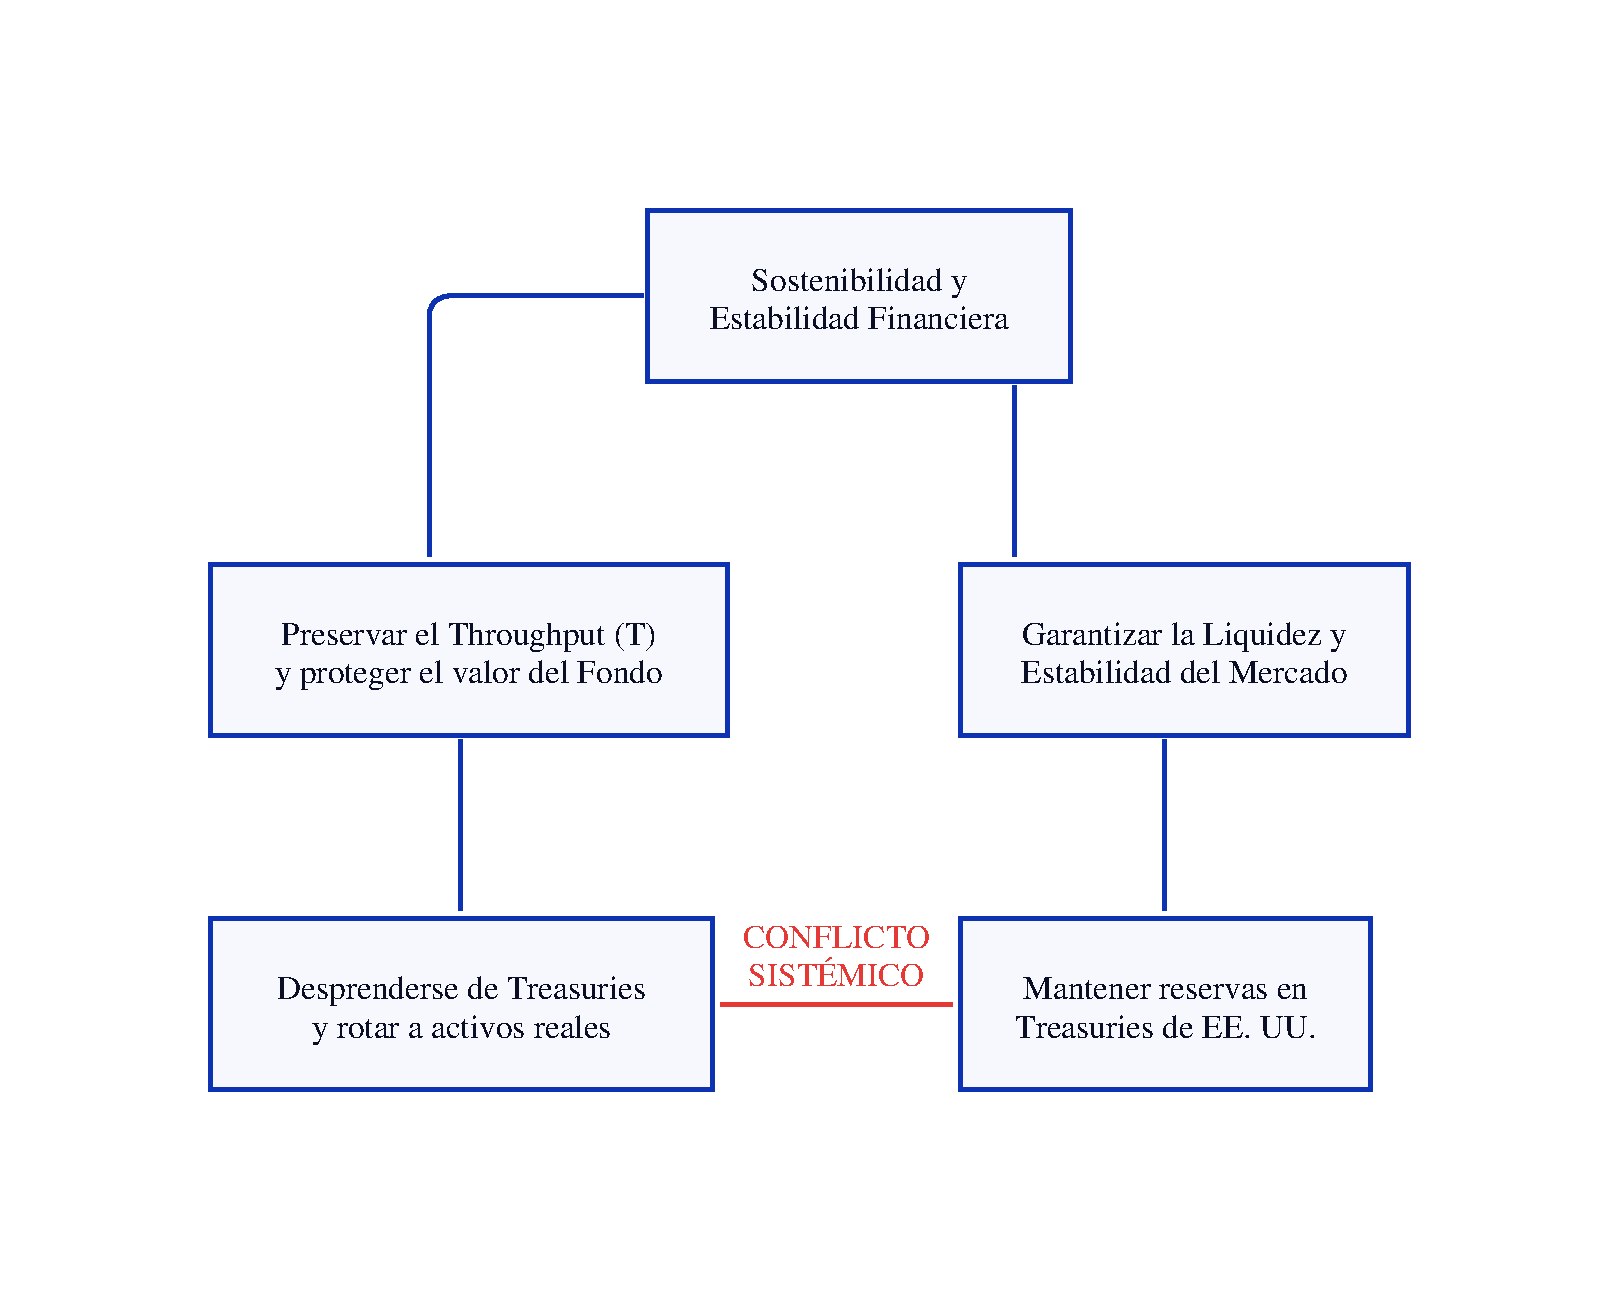
\includegraphics{Diagramas/nube-evaporacion-conflicto.pdf}
\caption{Nube de Evaporación del Conflicto (Evaporating Cloud)}
\end{figure}

\begin{itemize}
\tightlist
\item
  \textbf{Premisa Falsa Evaporada:} \emph{``Los U.S. Treasuries son el
  único activo infinitamente líquido y exento de riesgo de mercado para
  la reserva de capitales soberanos.''}
\item
  \textbf{Inyección TOC:} La sustitución de deuda gubernamental por
  crédito corporativo, hipotecas (\emph{MBS}) y activos reales genera
  mayor Throughput sin comprometer la liquidez operativa requerida por
  los fondos soberanos.
\end{itemize}

\begin{center}\rule{0.5\linewidth}{0.5pt}\end{center}

\hypertarget{dicotomuxeda-clave-1-contabilidad-de-costos-tradicional-vs.-contabilidad-del-throughput-ta}{%
\subsection{3. Dicotomía Clave 1: Contabilidad de Costos Tradicional
vs.~Contabilidad del Throughput
(TA)}\label{dicotomuxeda-clave-1-contabilidad-de-costos-tradicional-vs.-contabilidad-del-throughput-ta}}

\begin{longtable}[]{@{}
  >{\raggedright\arraybackslash}p{(\columnwidth - 4\tabcolsep) * \real{0.3333}}
  >{\raggedright\arraybackslash}p{(\columnwidth - 4\tabcolsep) * \real{0.3333}}
  >{\raggedright\arraybackslash}p{(\columnwidth - 4\tabcolsep) * \real{0.3333}}@{}}
\toprule\noalign{}
\begin{minipage}[b]{\linewidth}\raggedright
Enfoque
\end{minipage} & \begin{minipage}[b]{\linewidth}\raggedright
Interpretación de la Noticia
\end{minipage} & \begin{minipage}[b]{\linewidth}\raggedright
Impacto en la Toma de Decisiones
\end{minipage} \\
\midrule\noalign{}
\endhead
\bottomrule\noalign{}
\endlastfoot
\textbf{Contabilidad de Costos Tradicional} & Evalúa la movilización de
capital como una búsqueda de ``optimización de retornos locales''.
Recomienda diversificar asignaciones basándose en volatilidades
históricas y métricas de riesgo/retorno individuales (\emph{Sharpe
Ratio}). & Trata cada clase de activo de forma aislada, ignorando que la
venta masiva de \emph{Treasuries} incrementa el costo del capital global
(\textbf{OE}), encareciendo el financiamiento para las corporaciones
donde el mismo fondo posee acciones. \\
\textbf{Contabilidad del Throughput (TA)} & Identifica que retener deuda
soberana en desprecio de su poder adquisitivo paraliza el valor del
sistema. Entiende que el bono del Tesoro ha dejado de ser un activo
``seguro'' para convertirse en ``Inventario Atrapado'' (\textbf{I}). &
Prioriza proteger el flujo general (\textbf{T}). Si el canal primario de
liquidez destruye \textbf{T} debido a la inflación e inestabilidad de
tasas, la reasignación hacia activos con flujo real subyacente es
imperativa para la supervivencia del sistema. \\
\end{longtable}

\begin{center}\rule{0.5\linewidth}{0.5pt}\end{center}

\hypertarget{dicotomuxeda-clave-2-teoruxeda-monetaria-moderna-mmt-vs.-teoruxeda-de-restricciones-toc}{%
\subsection{4. Dicotomía Clave 2: Teoría Monetaria Moderna (MMT)
vs.~Teoría de Restricciones
(TOC)}\label{dicotomuxeda-clave-2-teoruxeda-monetaria-moderna-mmt-vs.-teoruxeda-de-restricciones-toc}}

\hypertarget{visiuxf3n-mmt}{%
\subsubsection{\texorpdfstring{\textbf{Visión
MMT:}}{Visión MMT:}}\label{visiuxf3n-mmt}}

Para la MMT, la liquidación de \$160 billones de dólares en
\emph{Treasuries} por parte de Noruega y Japón es un ajuste meramente
nominal de reservas. Dado que EE. UU. posee soberanía monetaria, el
gasto federal y el servicio de la deuda no enfrentan restricciones
financieras reales; el gobierno de EE. UU. siempre puede acreditar
cuentas bancarias y la Reserva Federal absorber la deuda no demandada.

\hypertarget{visiuxf3n-toc}{%
\subsubsection{\texorpdfstring{\textbf{Visión
TOC:}}{Visión TOC:}}\label{visiuxf3n-toc}}

El dinero es un simple habilitador del flujo, no la restricción. La
verdadera restricción es la \textbf{capacidad del sistema económico real
para absorber pasivos sin que el rendimiento exigido estrangule la
producción}. Si el mercado privado rechaza absorber el exceso de
``Inventario'' de deuda que dejan Noruega y Japón sin exigir
\emph{yields} drásticamente más altos, el costo de oportunidad destruirá
el Throughput (\textbf{T}) de la economía productiva. La inyección de
liquidez ilimitada mediante monetización (Fed) solo incrementa el
\emph{Ruido} y el \textbf{I} monetario, acelerando la pérdida de poder
de compra.

\begin{center}\rule{0.5\linewidth}{0.5pt}\end{center}

\hypertarget{conclusiuxf3n-y-prescripciuxf3n-estratuxe9gica-los-5-pasos-de-enfoque-de-goldratt}{%
\subsection{5. Conclusión y Prescripción Estratégica (Los 5 Pasos de
Enfoque de
Goldratt)}\label{conclusiuxf3n-y-prescripciuxf3n-estratuxe9gica-los-5-pasos-de-enfoque-de-goldratt}}

Para evitar un estrangulamiento del mercado de capitales global, el
sistema debe gestionar la restricción de absorción de deuda mediante los
cinco pasos iterativos:

\begin{enumerate}
\def\labelenumi{\arabic{enumi}.}
\tightlist
\item
  \textbf{IDENTIFICAR la Restricción:} Reconocer formalmente que la
  restricción del sistema financiero global es la capacidad limitada de
  los mercados para absorber déficit soberano sin disparar las tasas de
  interés reales.
\item
  \textbf{EXPLOTAR la Restricción:} Maximizar la eficiencia de la deuda
  existente. Los emisores soberanos (Tesoro de EE. UU.) deben
  reestructurar la durabilidad de sus emisiones (emitir en tramos de la
  curva de rendimientos con mayor demanda privada real) para optimizar
  el Throughput de absorción por dólar emitido.
\item
  \textbf{SUBORDINAR todo lo demás a la Restricción:} Alinear las
  políticas presupuestarias y monetarias. Los gobiernos deben
  disciplinar la expansión del gasto no productivo (\textbf{OE}) para no
  saturar con ``Inventario de Deuda'' innecesario el cuello de botella
  del mercado.
\item
  \textbf{ELEVAR la Restricción:} Desarrollar y profundizar canales
  alternativos de absorción de capitales y crédito privado (deuda de
  infraestructura, activos tangibles, mercados de renta fija
  corporativa) para que la liquidez global no dependa exclusivamente del
  canal del Tesoro estadounidense.
\item
  \textbf{PREVENIR la Inercia (Si la restricción se ha movido, volver al
  Paso 1):} Evitar el dogma de que los bonos soberanos son el único
  colateral libre de riesgo. Si la restricción migra desde el mercado de
  deuda pública hacia la solvencia del sistema bancario privado debido a
  las altas tasas, el modelo de gestión de riesgo global debe
  recalibrarse de inmediato.
\end{enumerate}

\end{document}
